\documentclass{standalone}
\usepackage{tikz}
\usetikzlibrary{patterns, positioning}


\begin{document}
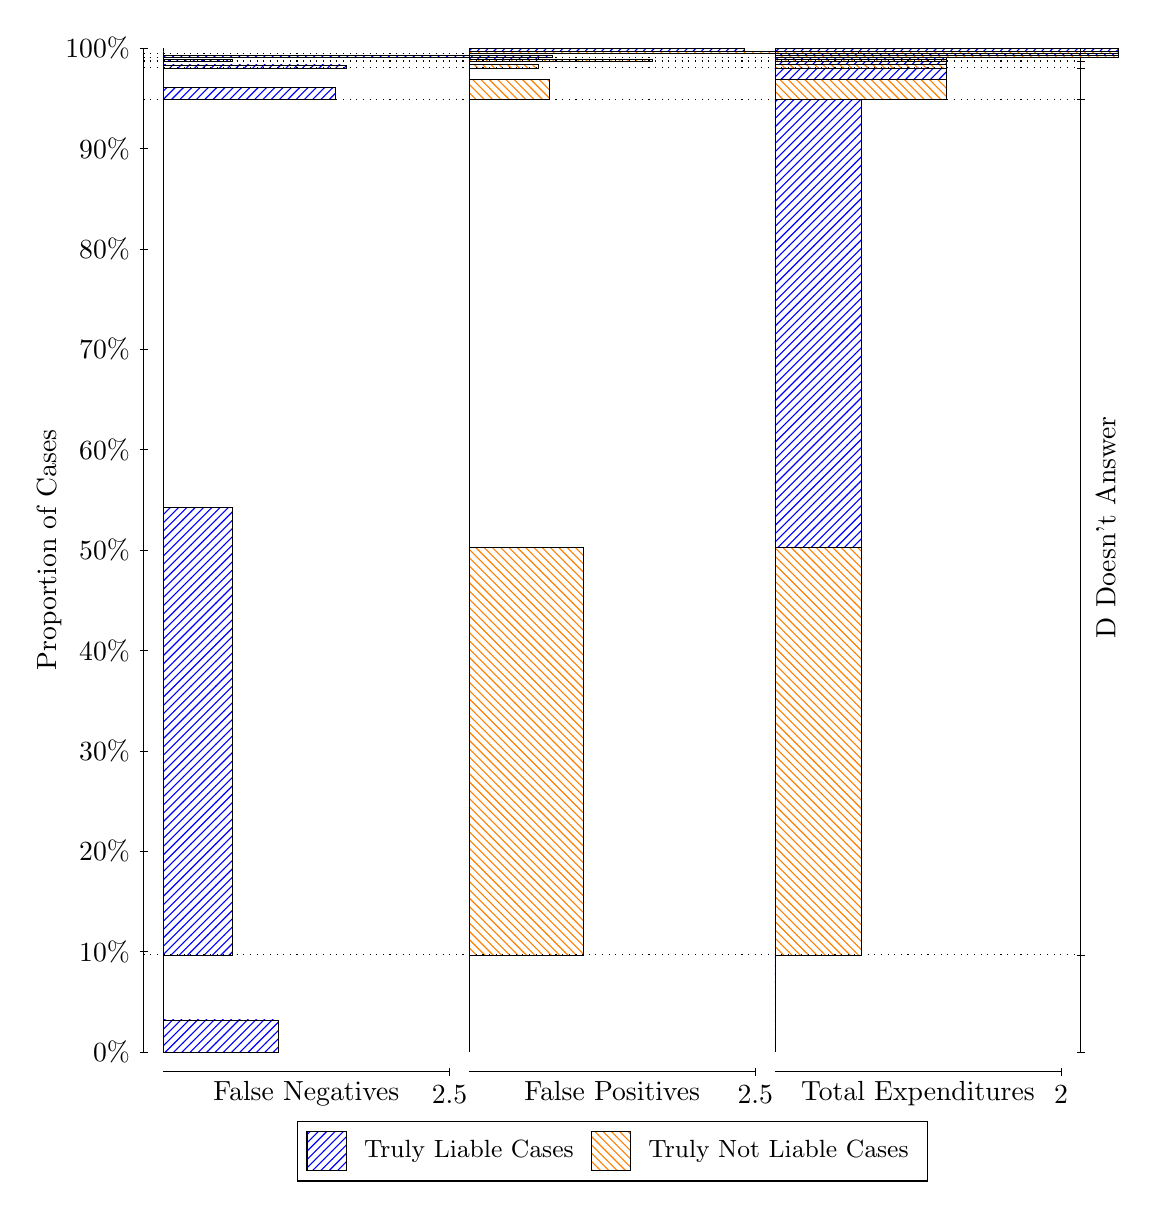
\begin{tikzpicture}
\draw[black, very thin] (1.5,1.75) -- (1.5,14.5);
\node[rotate=90, text=black, anchor=center] at (0.3, 8.125) {Proportion of Cases};
\draw[black, very thin] (1.45,1.75) -- (1.55,1.75);
\node[text=black, anchor=east] at (1.45, 1.75) {0\%};
\draw[black, very thin] (1.45,3.025) -- (1.55,3.025);
\node[text=black, anchor=east] at (1.45, 3.025) {10\%};
\draw[black, very thin] (1.45,4.3) -- (1.55,4.3);
\node[text=black, anchor=east] at (1.45, 4.3) {20\%};
\draw[black, very thin] (1.45,5.575) -- (1.55,5.575);
\node[text=black, anchor=east] at (1.45, 5.575) {30\%};
\draw[black, very thin] (1.45,6.85) -- (1.55,6.85);
\node[text=black, anchor=east] at (1.45, 6.85) {40\%};
\draw[black, very thin] (1.45,8.125) -- (1.55,8.125);
\node[text=black, anchor=east] at (1.45, 8.125) {50\%};
\draw[black, very thin] (1.45,9.4) -- (1.55,9.4);
\node[text=black, anchor=east] at (1.45, 9.4) {60\%};
\draw[black, very thin] (1.45,10.675) -- (1.55,10.675);
\node[text=black, anchor=east] at (1.45, 10.675) {70\%};
\draw[black, very thin] (1.45,11.95) -- (1.55,11.95);
\node[text=black, anchor=east] at (1.45, 11.95) {80\%};
\draw[black, very thin] (1.45,13.225) -- (1.55,13.225);
\node[text=black, anchor=east] at (1.45, 13.225) {90\%};
\draw[black, very thin] (1.45,14.5) -- (1.55,14.5);
\node[text=black, anchor=east] at (1.45, 14.5) {100\%};

\draw[black, very thin] (13.4,1.75) -- (13.4,14.5);
\draw[black, very thin] (13.35,1.75) -- (13.45,1.75);
\node[anchor=west] at (13.35, 1.75) {};
\draw[black, very thin] (13.35,2.9839) -- (13.45,2.9839);
\node[anchor=west] at (13.35, 2.9839) {};
\draw[black, very thin] (13.35,13.845) -- (13.45,13.845);
\node[anchor=west] at (13.35, 13.845) {};
\draw[black, very thin] (13.35,14.248) -- (13.45,14.248);
\node[anchor=west] at (13.35, 14.248) {};
\draw[black, very thin] (13.35,14.335) -- (13.45,14.335);
\node[anchor=west] at (13.35, 14.335) {};
\draw[black, very thin] (13.35,14.377) -- (13.45,14.377);
\node[anchor=west] at (13.35, 14.377) {};
\draw[black, very thin] (13.35,14.435) -- (13.45,14.435);
\node[anchor=west] at (13.35, 14.435) {};
\draw[black, very thin] (13.35,14.5) -- (13.45,14.5);
\node[anchor=west] at (13.35, 14.5) {};

\draw[black, very thin, pattern color=blue, pattern=north east lines] (1.75,1.75) rectangle (3.2033,2.1587);
\draw[black, very thin, pattern color=orange, pattern=north west lines] (1.75,2.1587) rectangle (1.75,2.9839);
\draw[black, very thin, pattern color=blue, pattern=north east lines] (1.75,2.9839) rectangle (2.622,8.6671);
\draw[black, very thin, pattern color=orange, pattern=north west lines] (1.75,8.6671) rectangle (1.75,13.845);
\draw[black, very thin, pattern color=blue, pattern=north east lines] (1.75,13.845) rectangle (3.93,13.996);
\draw[black, very thin, pattern color=orange, pattern=north west lines] (1.75,13.996) rectangle (1.75,14.248);
\draw[black, very thin, pattern color=blue, pattern=north east lines] (1.75,14.248) rectangle (4.0753,14.287);
\draw[black, very thin, pattern color=orange, pattern=north west lines] (1.75,14.287) rectangle (1.75,14.335);
\draw[black, very thin, pattern color=blue, pattern=north east lines] (1.75,14.335) rectangle (2.622,14.36);
\draw[black, very thin, pattern color=orange, pattern=north west lines] (1.75,14.36) rectangle (1.75,14.377);
\draw[black, very thin, pattern color=blue, pattern=north east lines] (1.75,14.377) rectangle (6.6913,14.402);
\draw[black, very thin, pattern color=orange, pattern=north west lines] (1.75,14.402) rectangle (1.75,14.435);
\draw[black, very thin, pattern color=orange, pattern=north west lines] (1.75,14.435) rectangle (1.75,14.456);
\draw[black, very thin, pattern color=blue, pattern=north east lines] (1.75,14.456) rectangle (1.75,14.5);
\draw[black, very thin, pattern color=orange, pattern=north west lines] (5.6333,1.75) rectangle (5.6333,2.5752);
\draw[black, very thin, pattern color=blue, pattern=north east lines] (5.6333,2.5752) rectangle (5.6333,2.9839);
\draw[black, very thin, pattern color=orange, pattern=north west lines] (5.6333,2.9839) rectangle (7.0867,8.1615);
\draw[black, very thin, pattern color=blue, pattern=north east lines] (5.6333,8.1615) rectangle (5.6333,13.845);
\draw[black, very thin, pattern color=orange, pattern=north west lines] (5.6333,13.845) rectangle (6.6507,14.097);
\draw[black, very thin, pattern color=blue, pattern=north east lines] (5.6333,14.097) rectangle (5.6333,14.248);
\draw[black, very thin, pattern color=orange, pattern=north west lines] (5.6333,14.248) rectangle (6.5053,14.296);
\draw[black, very thin, pattern color=blue, pattern=north east lines] (5.6333,14.296) rectangle (5.6333,14.335);
\draw[black, very thin, pattern color=orange, pattern=north west lines] (5.6333,14.335) rectangle (7.9587,14.352);
\draw[black, very thin, pattern color=blue, pattern=north east lines] (5.6333,14.352) rectangle (6.5053,14.377);
\draw[black, very thin, pattern color=orange, pattern=north west lines] (5.6333,14.377) rectangle (5.6333,14.41);
\draw[black, very thin, pattern color=blue, pattern=north east lines] (5.6333,14.41) rectangle (5.6333,14.435);
\draw[black, very thin, pattern color=orange, pattern=north west lines] (5.6333,14.435) rectangle (10.575,14.456);
\draw[black, very thin, pattern color=blue, pattern=north east lines] (5.6333,14.456) rectangle (9.1213,14.5);
\draw[black, very thin, pattern color=orange, pattern=north west lines] (9.5167,1.75) rectangle (9.5167,2.5752);
\draw[black, very thin, pattern color=blue, pattern=north east lines] (9.5167,2.5752) rectangle (9.5167,2.9839);
\draw[black, very thin, pattern color=orange, pattern=north west lines] (9.5167,2.9839) rectangle (10.607,8.1615);
\draw[black, very thin, pattern color=blue, pattern=north east lines] (9.5167,8.1615) rectangle (10.607,13.845);
\draw[black, very thin, pattern color=orange, pattern=north west lines] (9.5167,13.845) rectangle (11.697,14.097);
\draw[black, very thin, pattern color=blue, pattern=north east lines] (9.5167,14.097) rectangle (11.697,14.248);
\draw[black, very thin, pattern color=orange, pattern=north west lines] (9.5167,14.248) rectangle (11.697,14.296);
\draw[black, very thin, pattern color=blue, pattern=north east lines] (9.5167,14.296) rectangle (11.697,14.335);
\draw[black, very thin, pattern color=orange, pattern=north west lines] (9.5167,14.335) rectangle (11.697,14.352);
\draw[black, very thin, pattern color=blue, pattern=north east lines] (9.5167,14.352) rectangle (11.697,14.377);
\draw[black, very thin, pattern color=orange, pattern=north west lines] (9.5167,14.377) rectangle (13.877,14.41);
\draw[black, very thin, pattern color=blue, pattern=north east lines] (9.5167,14.41) rectangle (13.877,14.435);
\draw[black, very thin, pattern color=orange, pattern=north west lines] (9.5167,14.435) rectangle (13.877,14.456);
\draw[black, very thin, pattern color=blue, pattern=north east lines] (9.5167,14.456) rectangle (13.877,14.5);
\draw[black, dotted] (1.5,2.9839) -- (13.4,2.9839);
\draw[black, dotted] (1.5,13.845) -- (13.4,13.845);
\draw[black, dotted] (1.5,14.248) -- (13.4,14.248);
\draw[black, dotted] (1.5,14.335) -- (13.4,14.335);
\draw[black, dotted] (1.5,14.377) -- (13.4,14.377);
\draw[black, dotted] (1.5,14.435) -- (13.4,14.435);
\draw[black, very thin] (1.75,1.5) -- (5.3833,1.5);
\node[text=black, anchor=north] at (3.5667, 1.5) {False Negatives};
\draw[black, very thin] (5.3833,1.45) -- (5.3833,1.55);
\node[text=black, anchor=north] at (5.3833, 1.45) {2.5};

\draw[black, very thin] (5.6333,1.5) -- (9.2667,1.5);
\node[text=black, anchor=north] at (7.45, 1.5) {False Positives};
\draw[black, very thin] (9.2667,1.45) -- (9.2667,1.55);
\node[text=black, anchor=north] at (9.2667, 1.45) {2.5};

\draw[black, very thin] (9.5167,1.5) -- (13.15,1.5);
\node[text=black, anchor=north] at (11.333, 1.5) {Total Expenditures};
\draw[black, very thin] (13.15,1.45) -- (13.15,1.55);
\node[text=black, anchor=north] at (13.15, 1.45) {2};


\node[text=black, centered, rotate=90] at (13.72, 8.4143) {D Doesn't Answer};






\draw (7.449999999999999,1.5) node[draw=none] (baseCoordinate) {};
\begin{scope}[align=center]
        \matrix[scale=0.5, draw=black, below=0.5cm of baseCoordinate, nodes={draw}, column sep=0.1cm]{
            \node[rectangle, draw, minimum width=0.5cm, minimum height=0.5cm, pattern color=blue, pattern=north east lines] {}; &
            \node[draw=none, font=\small, text=black] (B) {Truly Liable Cases}; &
            \node[rectangle, draw, minimum width=0.5cm, minimum height=0.5cm, pattern color=orange, pattern=north west lines] {}; &
            \node[draw=none, font=\small, text=black] (B) {Truly Not Liable Cases}; \\
            };
\end{scope}

\end{tikzpicture}
\end{document}